% \documentclass[11pt,twoside,a4paper]{article}
\documentclass{article}

%package for utf-8 support
\usepackage[utf8]{inputenc}
\usepackage[backend=biber]{biblatex}
\addbibresource{ref.bib}

% \usepackage{cite}
% \usepackage{csquotes}


% A couple of useful packages
\usepackage[table]{xcolor}
\usepackage{listings}
\usepackage{color}
\usepackage{import} % Used for importing the pdf_tex from inckscape
\usepackage{graphics} % for pdf, bitmapped graphics files
\usepackage{epsfig} % for postscript graphics files
% \usepackage{mathptmx} % assumes new font selection scheme installed
% \usepackage{times} % assumes new font selection scheme installed
\usepackage{amsmath} % assumes amsmath package installed
\usepackage{amssymb}  % assumes amsmath package installed
% \usepackage{mdwmath}
% \usepackage{algorithm}
% \usepackage{algorithmic}
% \usepackage{multirow}
\usepackage[margin=2cm]{geometry}
\usepackage[final]{pdfpages}
% \usepackage{pdfpages}
\usepackage{acronym}
\usepackage{afterpage}
\usepackage{xargs}
\usepackage{todonotes}


% Package that forces figures to stay within the section.
\usepackage[section]{placeins}

% A way to write about nodes in the graph
\newcommandx{\node}[2]{\item[\textbf{#1}] \textbf{#2}}
\newcommandx{\Q}[1]{\item[ $Q_{#1}$ ] }
\newcommandx{\aruco}{ArUco}
\newcommandx{\openpose}{OpenPose }

% Adding math symbols for real numbers.
\newcommandx{\R}{\mathbb{R}}

\title{3D reconstruction of spatial skeletal model}
\author{Magnus Sörensen}
\date{2020 November}


\begin{document}
% \maketitle
% \acrodef{sysml}[SysML]{System modelling language}
% \acrodef{uml}[UML]{Unified Modeling Language}
% \acrodef{ar}[AR]{Artificial reality}
%%International Council on Systems Engineering (INCOSE)
%\acrodef{incose}[INCOSE]{International Council on Systems Engineering}
%%\acrodef{A}[B]{C}
%%\acrodef{A}[B]{C}
%%\acrodef{A}[B]{C}
%%\acrodef{A}[B]{C}
%% ------------------- From here to ------------------------------
\vspace{5cm}
\begin{center}

\includegraphics[width=\textwidth, keepaspectratio]{aruco_00.png}
\end{center}
\vspace{2cm}
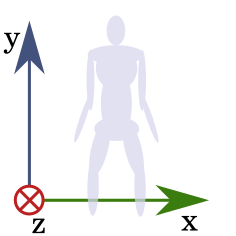
\includegraphics[width=3cm, keepaspectratio]{origin_fig.png}
\newpage
\myemptypage
\vspace{5cm}
\begin{center}

\includegraphics[width=\textwidth, keepaspectratio]{aruco_04.png}
\end{center}
\newpage
\myemptypage
\vspace{5cm}
\begin{center}

\includegraphics[width=\textwidth, keepaspectratio]{aruco_05.png}
\end{center}
\newpage
\myemptypage
\vspace{5cm}
\begin{center}

\includegraphics[width=\textwidth, keepaspectratio]{aruco_06.png}
\end{center}
\newpage
\myemptypage
\vspace{5cm}
\begin{center}

\includegraphics[width=\textwidth, keepaspectratio]{aruco_07.png}
\end{center}
\newpage
\myemptypage
\vspace{5cm}
\begin{center}

\includegraphics[width=\textwidth, keepaspectratio]{aruco_08.png}
\end{center}
\newpage
\myemptypage
\vspace{5cm}
\begin{center}

\includegraphics[width=\textwidth, keepaspectratio]{aruco_09.png}
\end{center}
\newpage
\myemptypage
\vspace{5cm}
\begin{center}

\includegraphics[width=\textwidth, keepaspectratio]{aruco_10.png}
\end{center}
\newpage
\myemptypage
\vspace{5cm}
\begin{center}

\includegraphics[width=\textwidth, keepaspectratio]{aruco_11.png}
\end{center}
\newpage
\myemptypage
\vspace{5cm}
\begin{center}
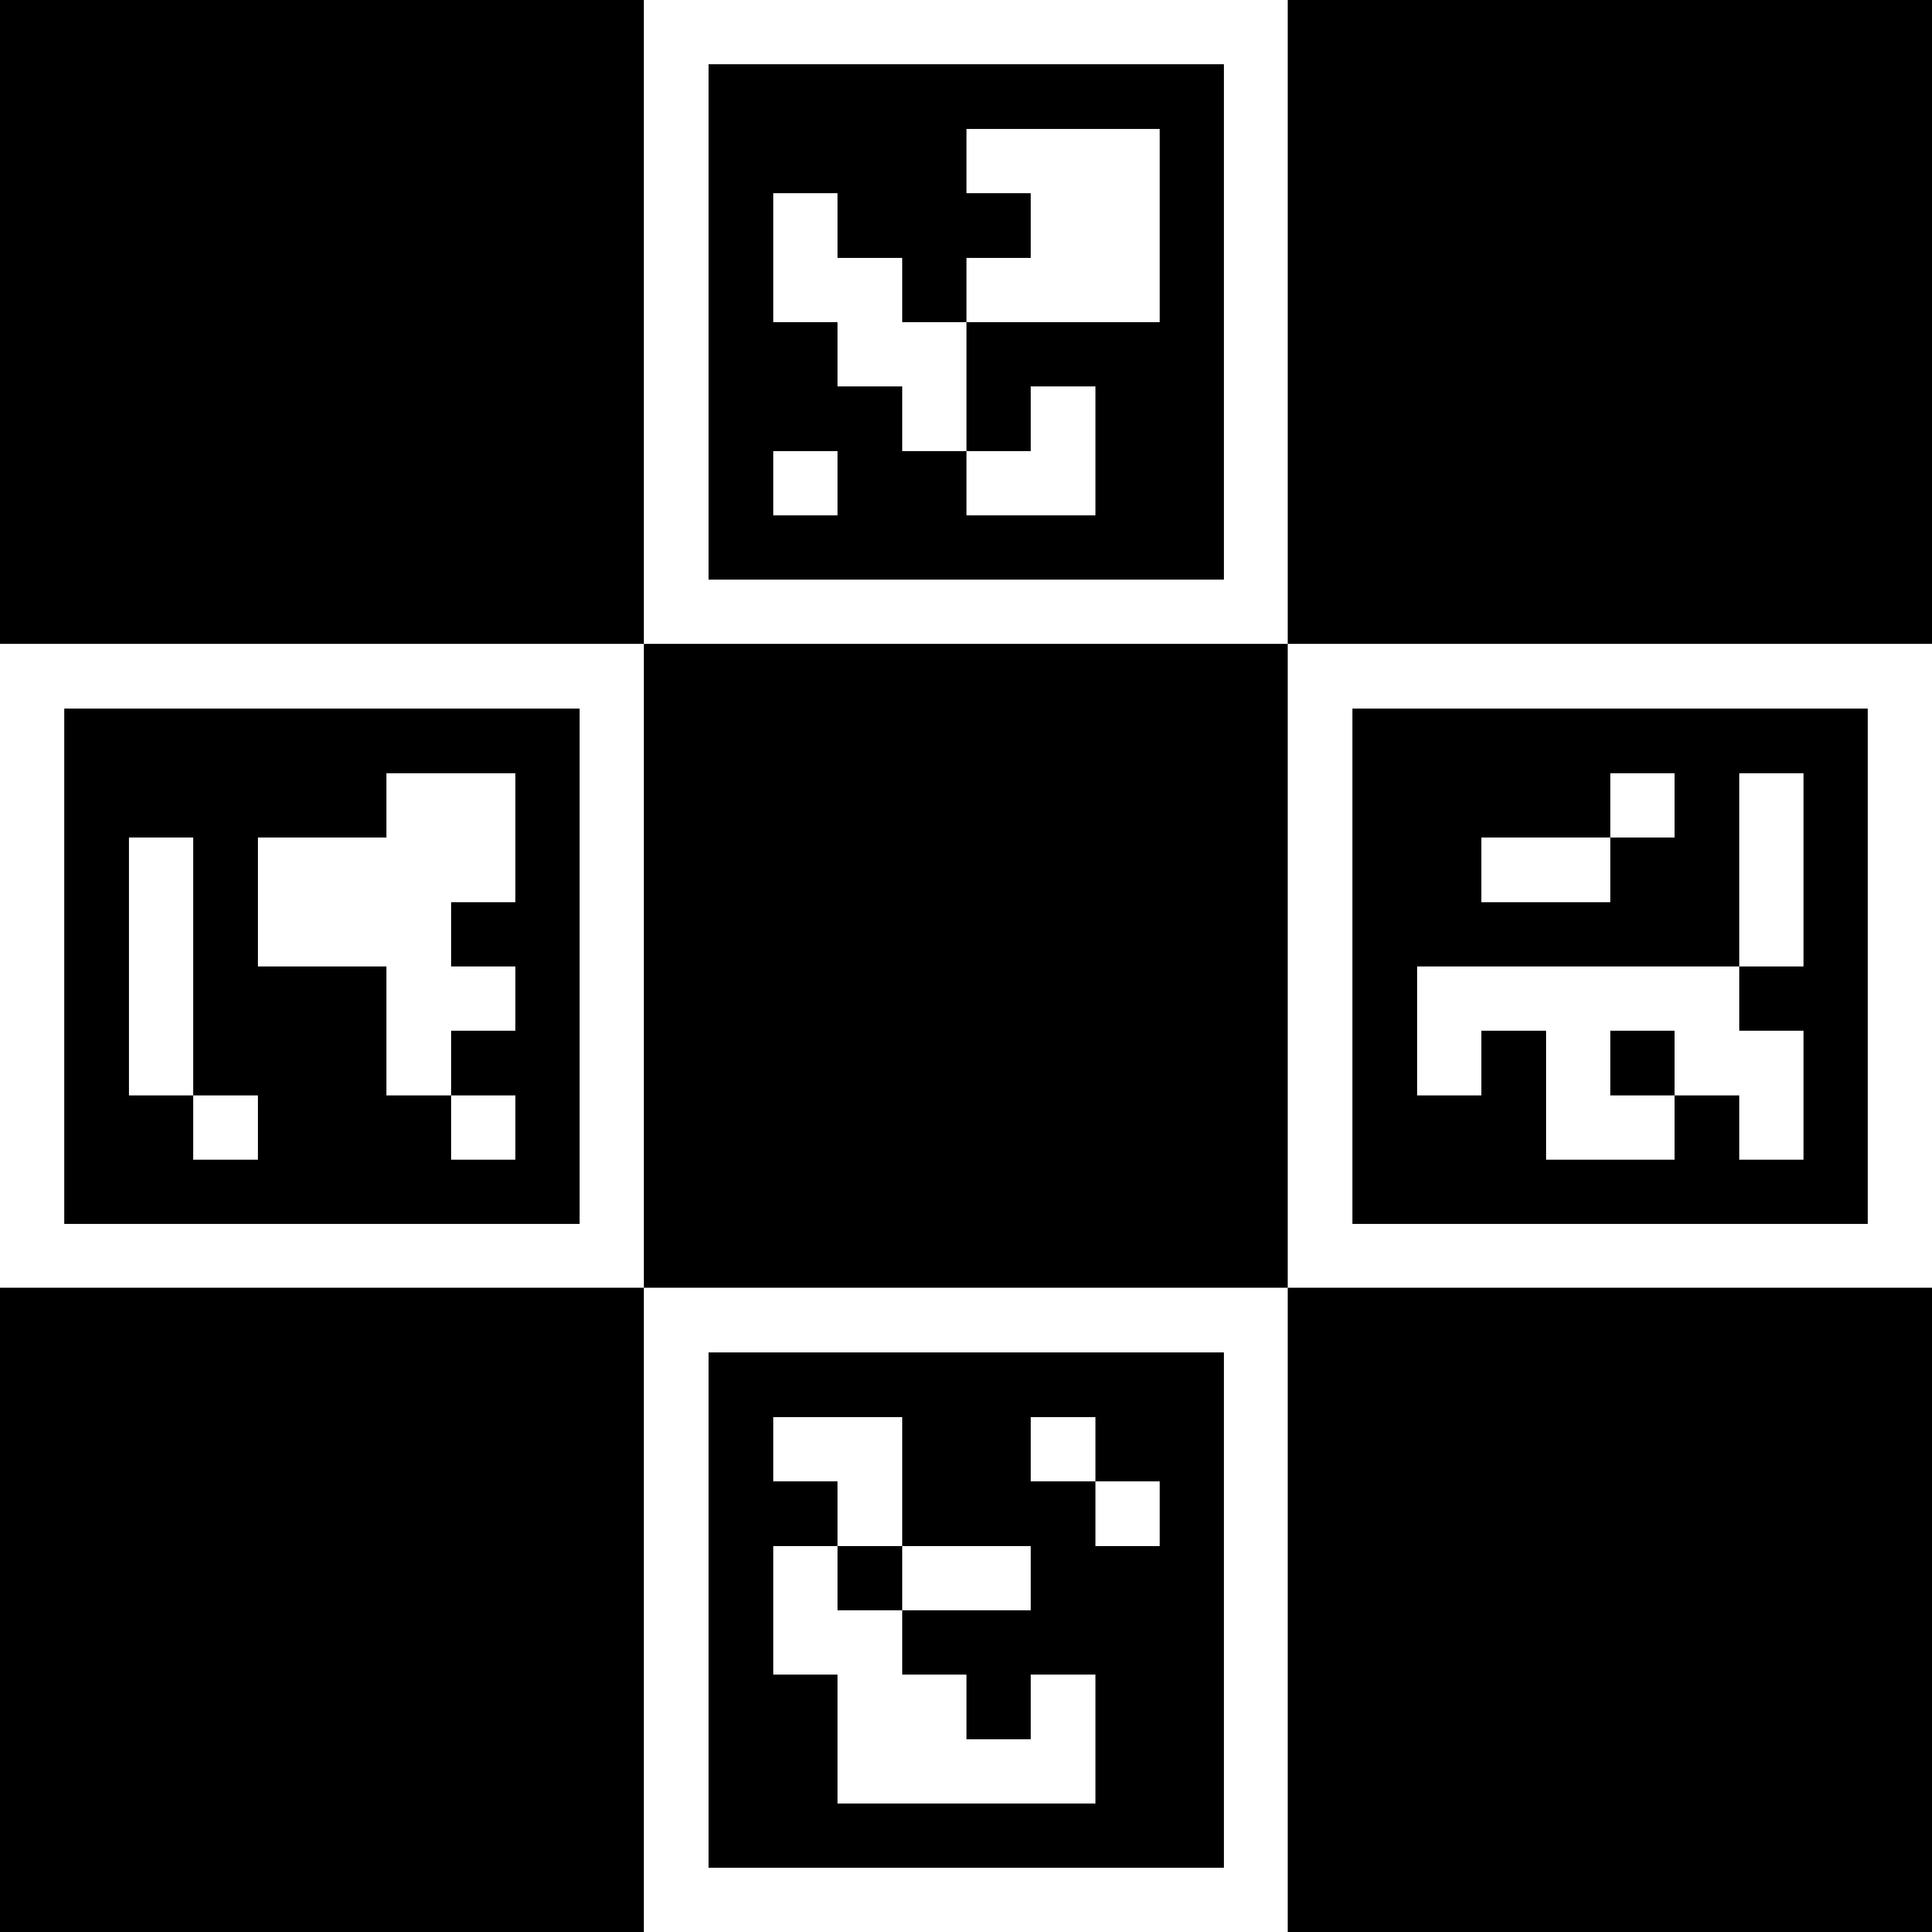
\includegraphics[width=\textwidth, keepaspectratio]{caruco_board.png}
\end{center}
\newpage
\myemptypage


% % \input{./10_introduction.tex}
% % The problem~\cite{moons20093d} uses \ac{ar}.
% % a new problem in~\cite{romero2018speeded}.
% \input{10_introduction.tex}
% \input{20_baground.tex}
% \input{30_implementation.tex}
% \input{40_method.tex}
% \printbibliography


% 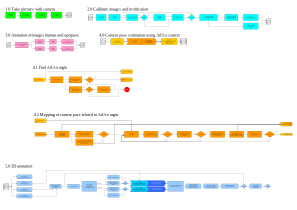
\includepdf[landscape=true]{Figures/planing.pdf}
% % \afterpage{\protect\crearpage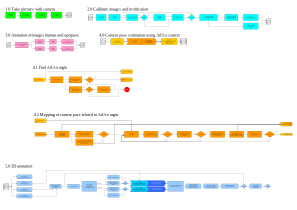
\includepdf[landscape=true]{Figures/planing.pdf}}
% % \afterpage{\crearpage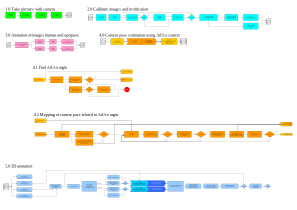
\includepdf[landscape=true]{Figures/planing.pdf}}
\end{document}


